\input{../std.tex}

\begin{document}
  \begin{center}
    \LARGE \textbf{Física Computacional} \\
    \Large \textbf{Tarefa 7 - Questão 5} \\
    \large Alex Enrique Crispim
  \end{center}

  Em contraste com a questão 4, podemos variar a amplitude da força induzida $F_d$. Um modo prático de fazer tal variação é criando um \textit{array} \texttt{Fd[]}, e iterando-se os índices do array, para poupar espaço no código.

  A modificação do programa utilizado na questão anterior se encontra no mesmo endreço de repositório no github, na pasta \textit{question 5}.

  A figura abaixo mostra o gráfico obtido para $F_d = 0.5$ e $F_d = 1.2$.

  \begin{figure}[h]
    \center
    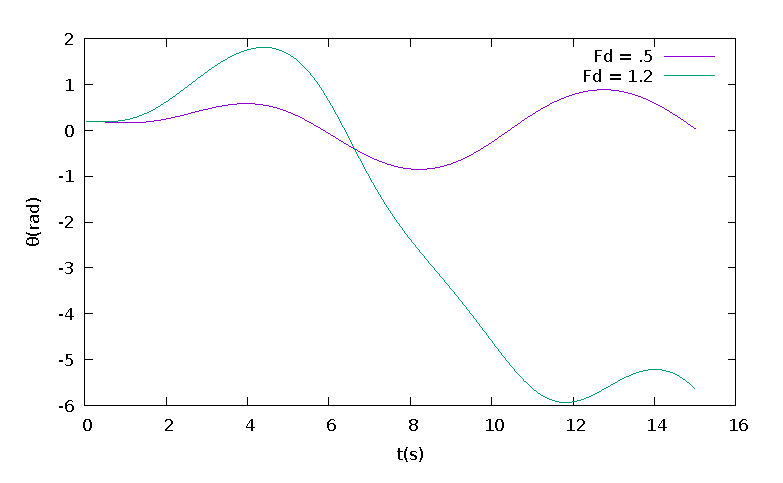
\includegraphics{q5Fig}
  \end{figure}


\end{document}
